%-------------------------------------------------------------------------------
\Section{Muon-based Accelerators} \par
Muons ($\mu$) were first discovered experimentally in 1947 by Powell et. al \cite{griffithspp} who were looking for the Yukawa meson.
It is now known that muons in fact fit into a fundamental particle group called leptons, and fit into the standard model as shown in Figure 1.

\begin{figure}[h!]
\label{fig:standardmodel}
\centering
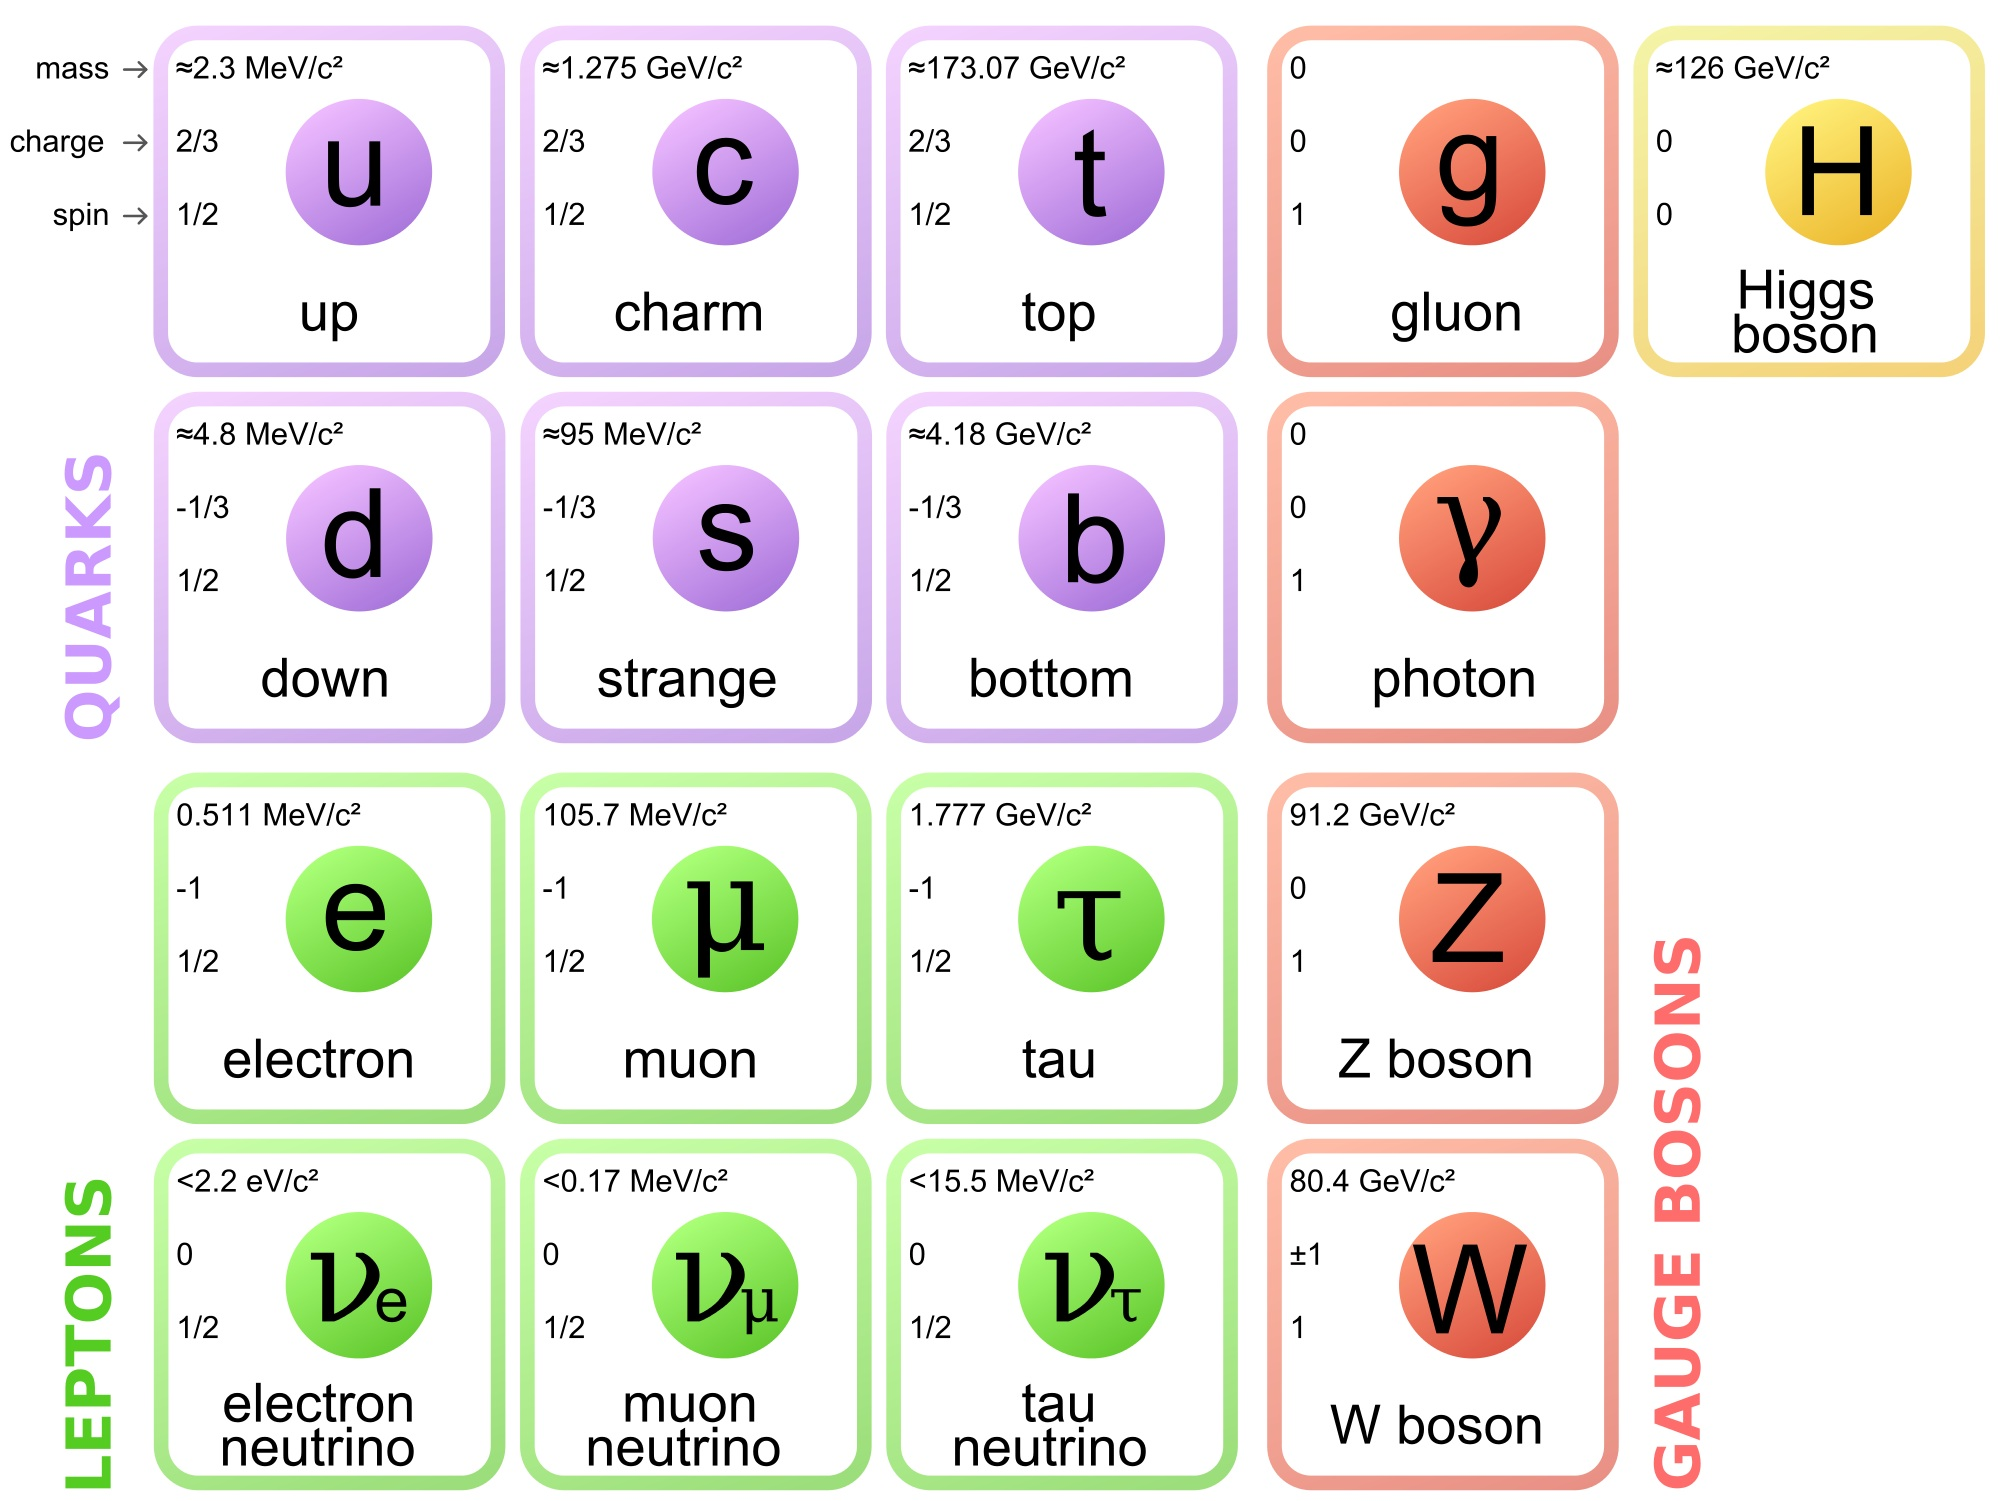
\includegraphics[width=0.8\textwidth]{Figures/standardmodel.jpg} 
 \caption{The current model of particle physics. Image courtesy of \cite{quantumdiaries}.}
\end{figure}

Similar to the electron ($e$), the muon carries a fundamental charge of $\pm$1, a spin of 1/2, and observes the electromagnetic and weak forces. Moreover, the muon also has a corresponding neutrino: the muon neutrino ($\nu_\mu$). However, the muon (mass = 105.7 MeV/$c^2$) is about 200 times heavier than the electron (mass = 0.511 MeV/$c^2$). Indeed, sometimes it is useful to think of a muon simply as a heavy electron, but the mass implies several unique characteristics. One of these are the instability of muons, since the following process is not forbidden by mass, charge, or lepton number conservation:
\begin{equation} \nonumber
\mu \rightarrow e+\bar{\nu_e}+\nu_\mu.\\
\end{equation}

This is quite interesting, as it means muons are a double-edged sword. On the one hand, their fundamentality means that the muon collisions will be clean. This is a great advantage over baryon collisions, since baryons are composed of three quarks (e.g. protons, neutrons). Consequently, any data from muon interactions will have relatively little noise and will not require the burden of jet analysis (as is sometimes the advantage of linear electron colliders). Yet unlike the electron, the muon does not emit a large amount of synchrotron radiation as it is accelerated. For this reason, it is possible to have a circular muon accelerator, and one far smaller than the equivalent baryon accelerator due to its small comparitive mass. On the other hand, a rest frame lifetime of 2 $\mu$s requires the muons to be accelerated before they decay. This is a challenge for circular colliders which require a high luminosity beam.

Now, it appears that there are several good advantages and only one disadvantage: the 2 $\mu$s mean rest frame lifetime of the muon. However, this is only a disadvantage for muon colliders. Another application which turns the moderately short lifetime into an advantage is that of a neutrino factory. The concept of a muon storage ring has existed since 1960 \cite{unpublishedring}, and its list of advantages only grows with time. 

%-------------------------------------------------------------------------------
\Section{COSY Infinity}\par
COSY Infinity is a beamline simulations tool used in the design, analysis, and optomization of particle accelerators \cite{cosy}. To do this, COSY uses the transfer map approach, which evaluates the overall effect of a system on a beam of particles  using differential algebra (involving multivariate Taylor polynomials up to arbitrary order). While a transfer map is technically not a nonlinear matrix, it is sometimes helpful to think of them as one in the same. Along with the evaluation of particles through a lattice, COSY also has a plethora of analysis and optomization tools, including (but not limited to) lattice aberration and correction tools, support for Twiss parameters, support for tunes and nonlinear tune shifts, built-in optimizers (for lattice design), and spin tracking. \par

COSY is particularly advantageous to use when considering the efficient use of computational time. This is due to the transfer map methods that COSY employs. Given some initial phase space vector $\mathbf{Z}(s_0)$ (see Figure \ref{fig:phaseSpaceVector}), the transfer map $\mathcal{M}$ will uniquely predict the time evolution of $\mathbf{Z}$. This is because most beam elements follow Maxwell's equations, which yield unique solutions that are dependent on initial conditions. Mathematically, this relationship is $\mathbf{Z}(s)=\mathcal{M}(s_0 , s)*\mathbf{Z}(s_0)$. Here, the independent variable $s$ is understood as the reference orbit (the zero point of a beam of particles in some comoving reference frame --see Figure \ref{fig:saxis}). An example of this relationship can be seen in Figure \ref{fig:matrix_element_example_1}. The initial phase space occupied by the beam of particles is at the coordinate $s_0$. Physically, there exists some deterministic beamline element. This element can be represented by the map $\mathcal{M}$, which creates a bijection for the phase space vectors $Z(s_0)$ and $Z(s)$ between the initial coordinate $s_0$ and an arbitrary final coordinate $s$. 

Valid elements are any beamline tools which are deterministic. Elements used in this study are magnetic multipoles (dipoles, quadrupoles, etc.), RF cavities, and drifts. Currently supported elements in COSY include but are not limited to: various magnetic and electric multipoles (with fringing effects), homogeneous and inhomogeneous bending elements, Wien filters, wigglers and undulators, cavities, cylindrical electromagnetic lenses, general particle optical elements, and deterministic polynomial absorbers of arbitrary order, with the last element being of particular interest.

\begin{figure}[h!]
\centering
$\mathbf{Z}=
\begin{pmatrix}
x\\ y\\ l=k(t-t_0)\\a=p_x/p_0\\b=p_y/p_0\\  \delta = (E-E_0)/E_0
\end{pmatrix}
$
\caption{Phase space vector $\mathbf{Z}$. Coordinates are transverse positions ($x, y$), time-of-flight in units of length ($l$), transverse angles w.r.t. the reference particle ($a, b$), and kinetic energy deviations w.r.t. the reference particle ($\delta$). The $0$ subscript in the definitions denotes the reference particle's properties.}
\label{fig:phaseSpaceVector}
\end{figure}

\begin{figure}[h!]
\centering
\includegraphics*[width=70mm]{./Figures/saxis}
\caption{The reference orbit.}
\label{fig:saxis}
\end{figure}


\begin{figure}[h!]
  \centering
    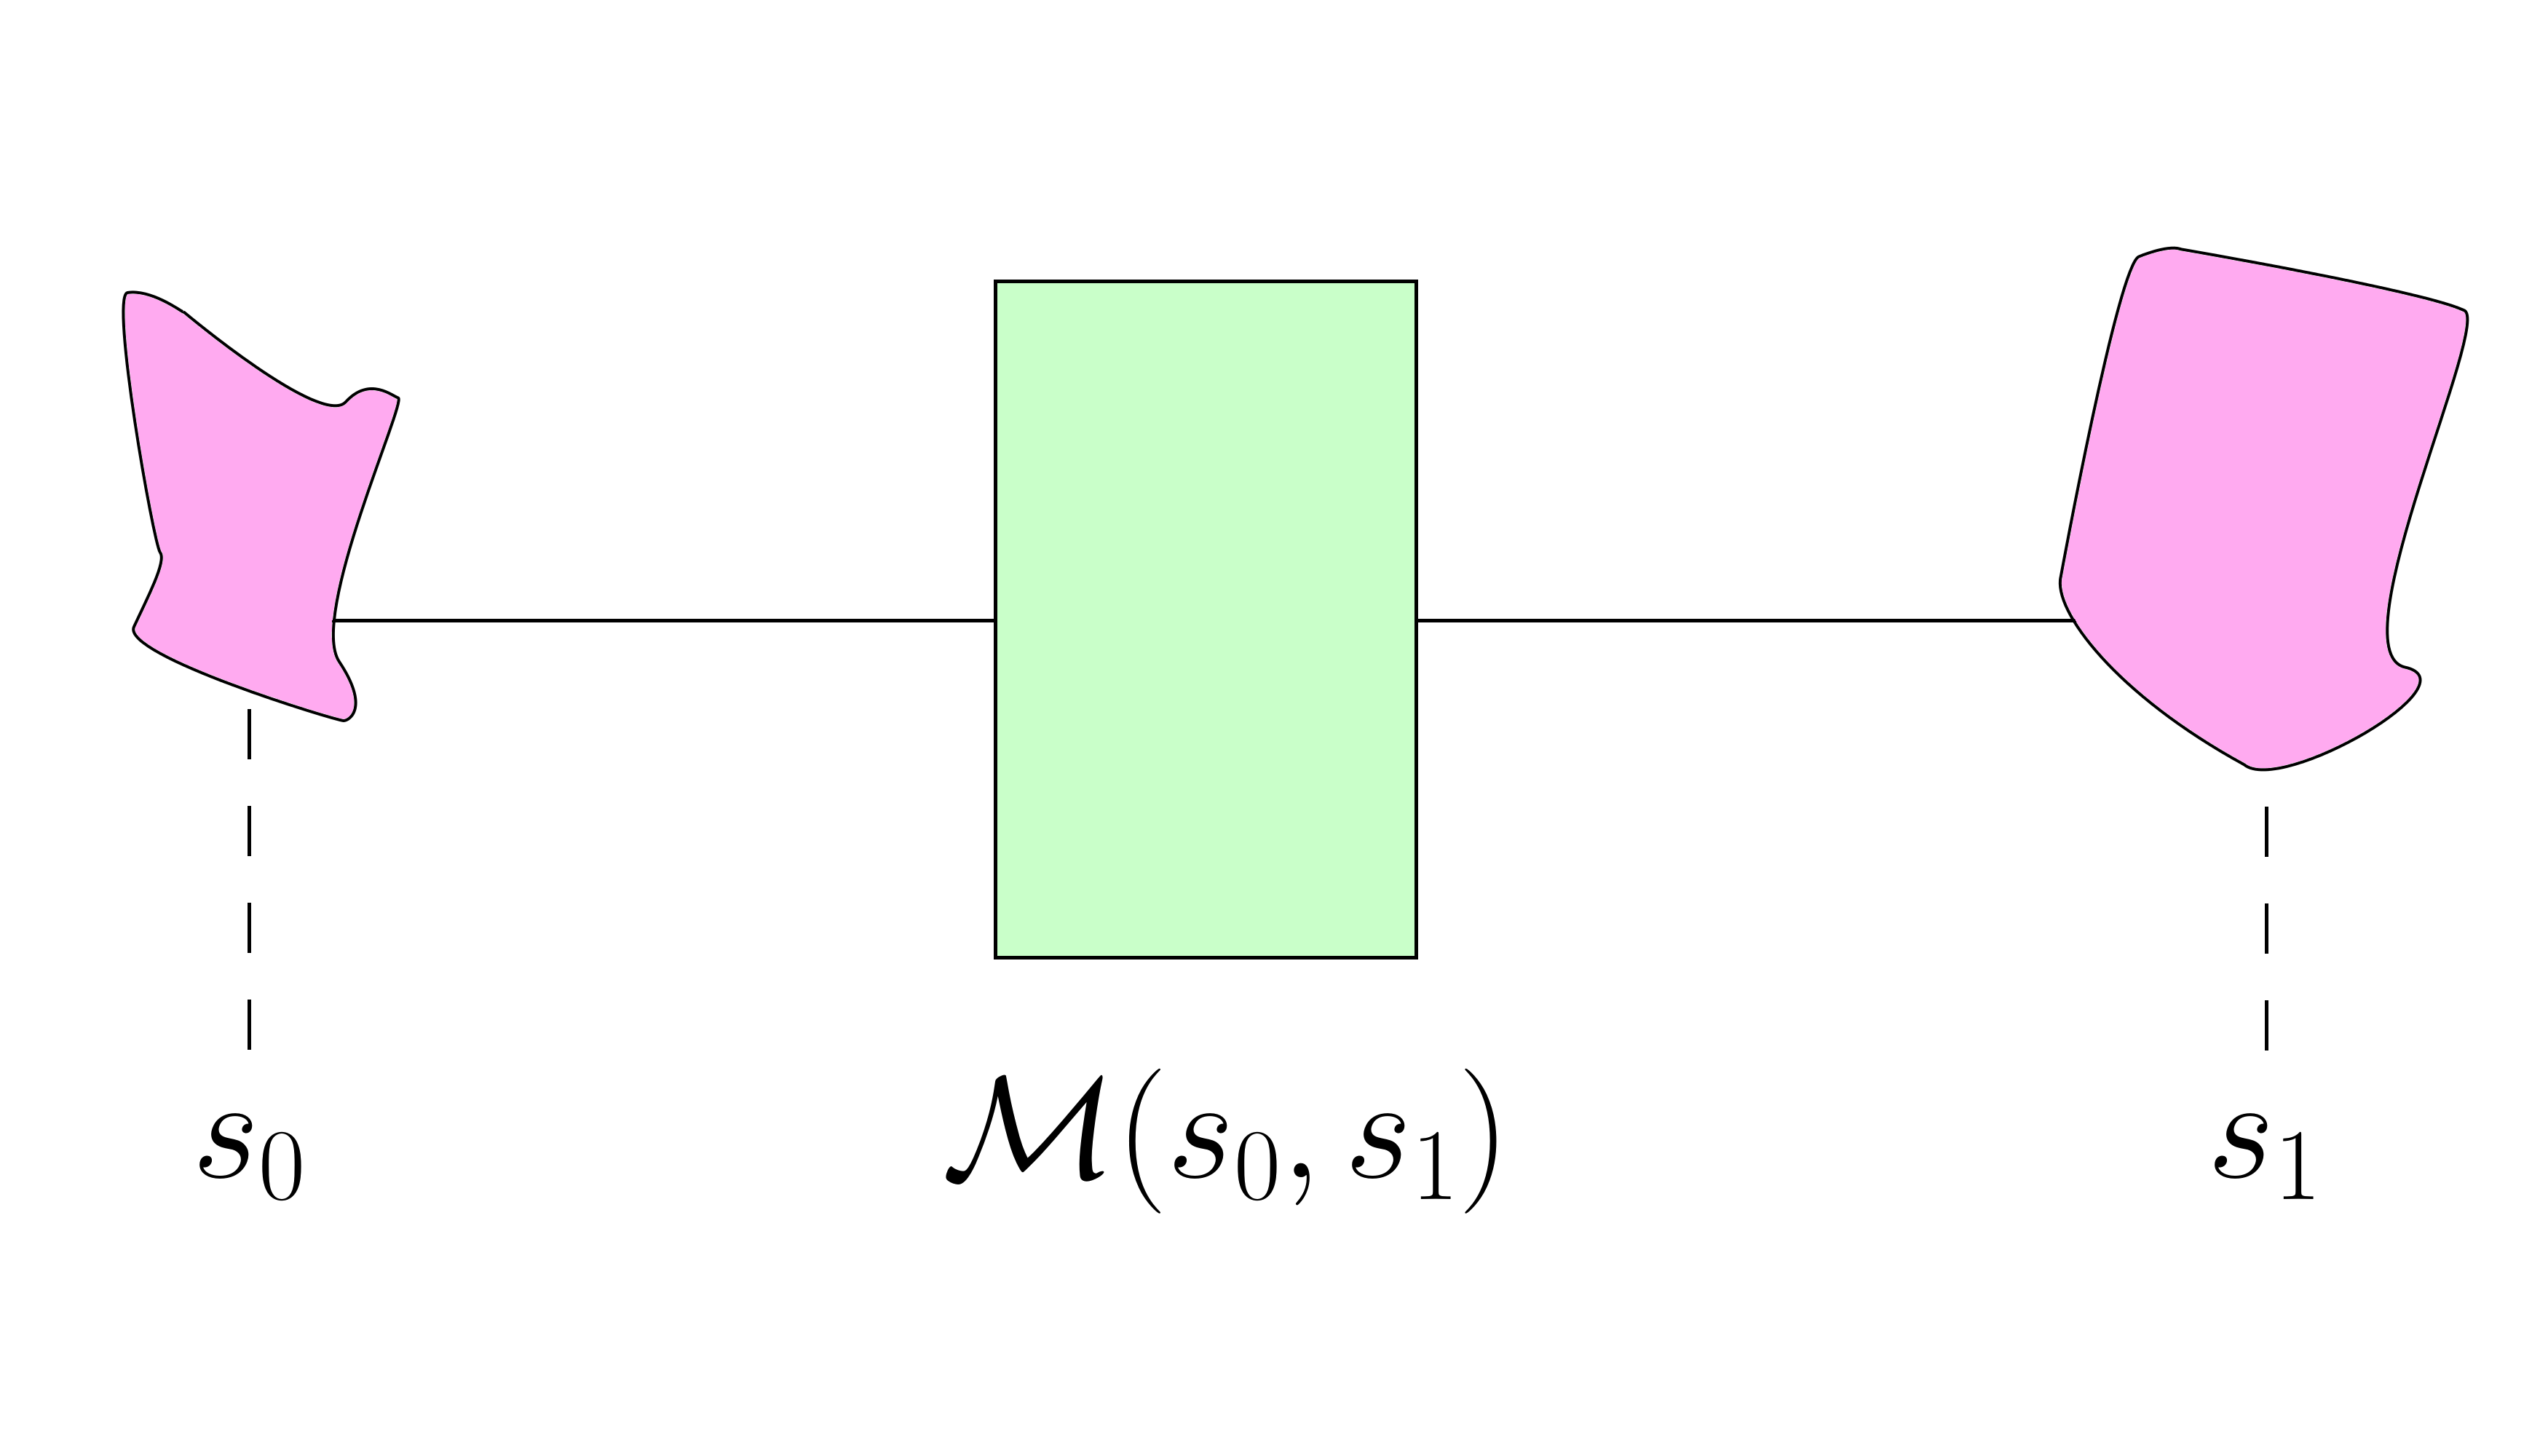
\includegraphics[width=0.75\textwidth]{Figures/matrix_element_example_1} 
  \caption{Example of some map $\mathcal{M}$ creating a bijection from $s_0$ to $s_1$.}
  \label{fig:matrix_element_example_1}
\end{figure}

Now, the composition of two maps yeilds another map: $\mathcal{M}(s_1 , s_2)\times \mathcal{M}(s_0 , s_1) = \mathcal{M}(s_0 , s_2)$. Therefore, it is possible to ``cut out" the middle part $s_1$. Since each physical lattice corresponds to some transfer map, it is possible to construct a single map that represents many individual lattices. An example of this can be seen in Figure \ref{fig:matrix_element_example_2}. Computationally this is advantageous because once calculated, it is much faster to apply a solitary transfer map to a distribution of particles than to simulate that same distribution through many meters of lattices.
\begin{figure}[h!]
  \centering
    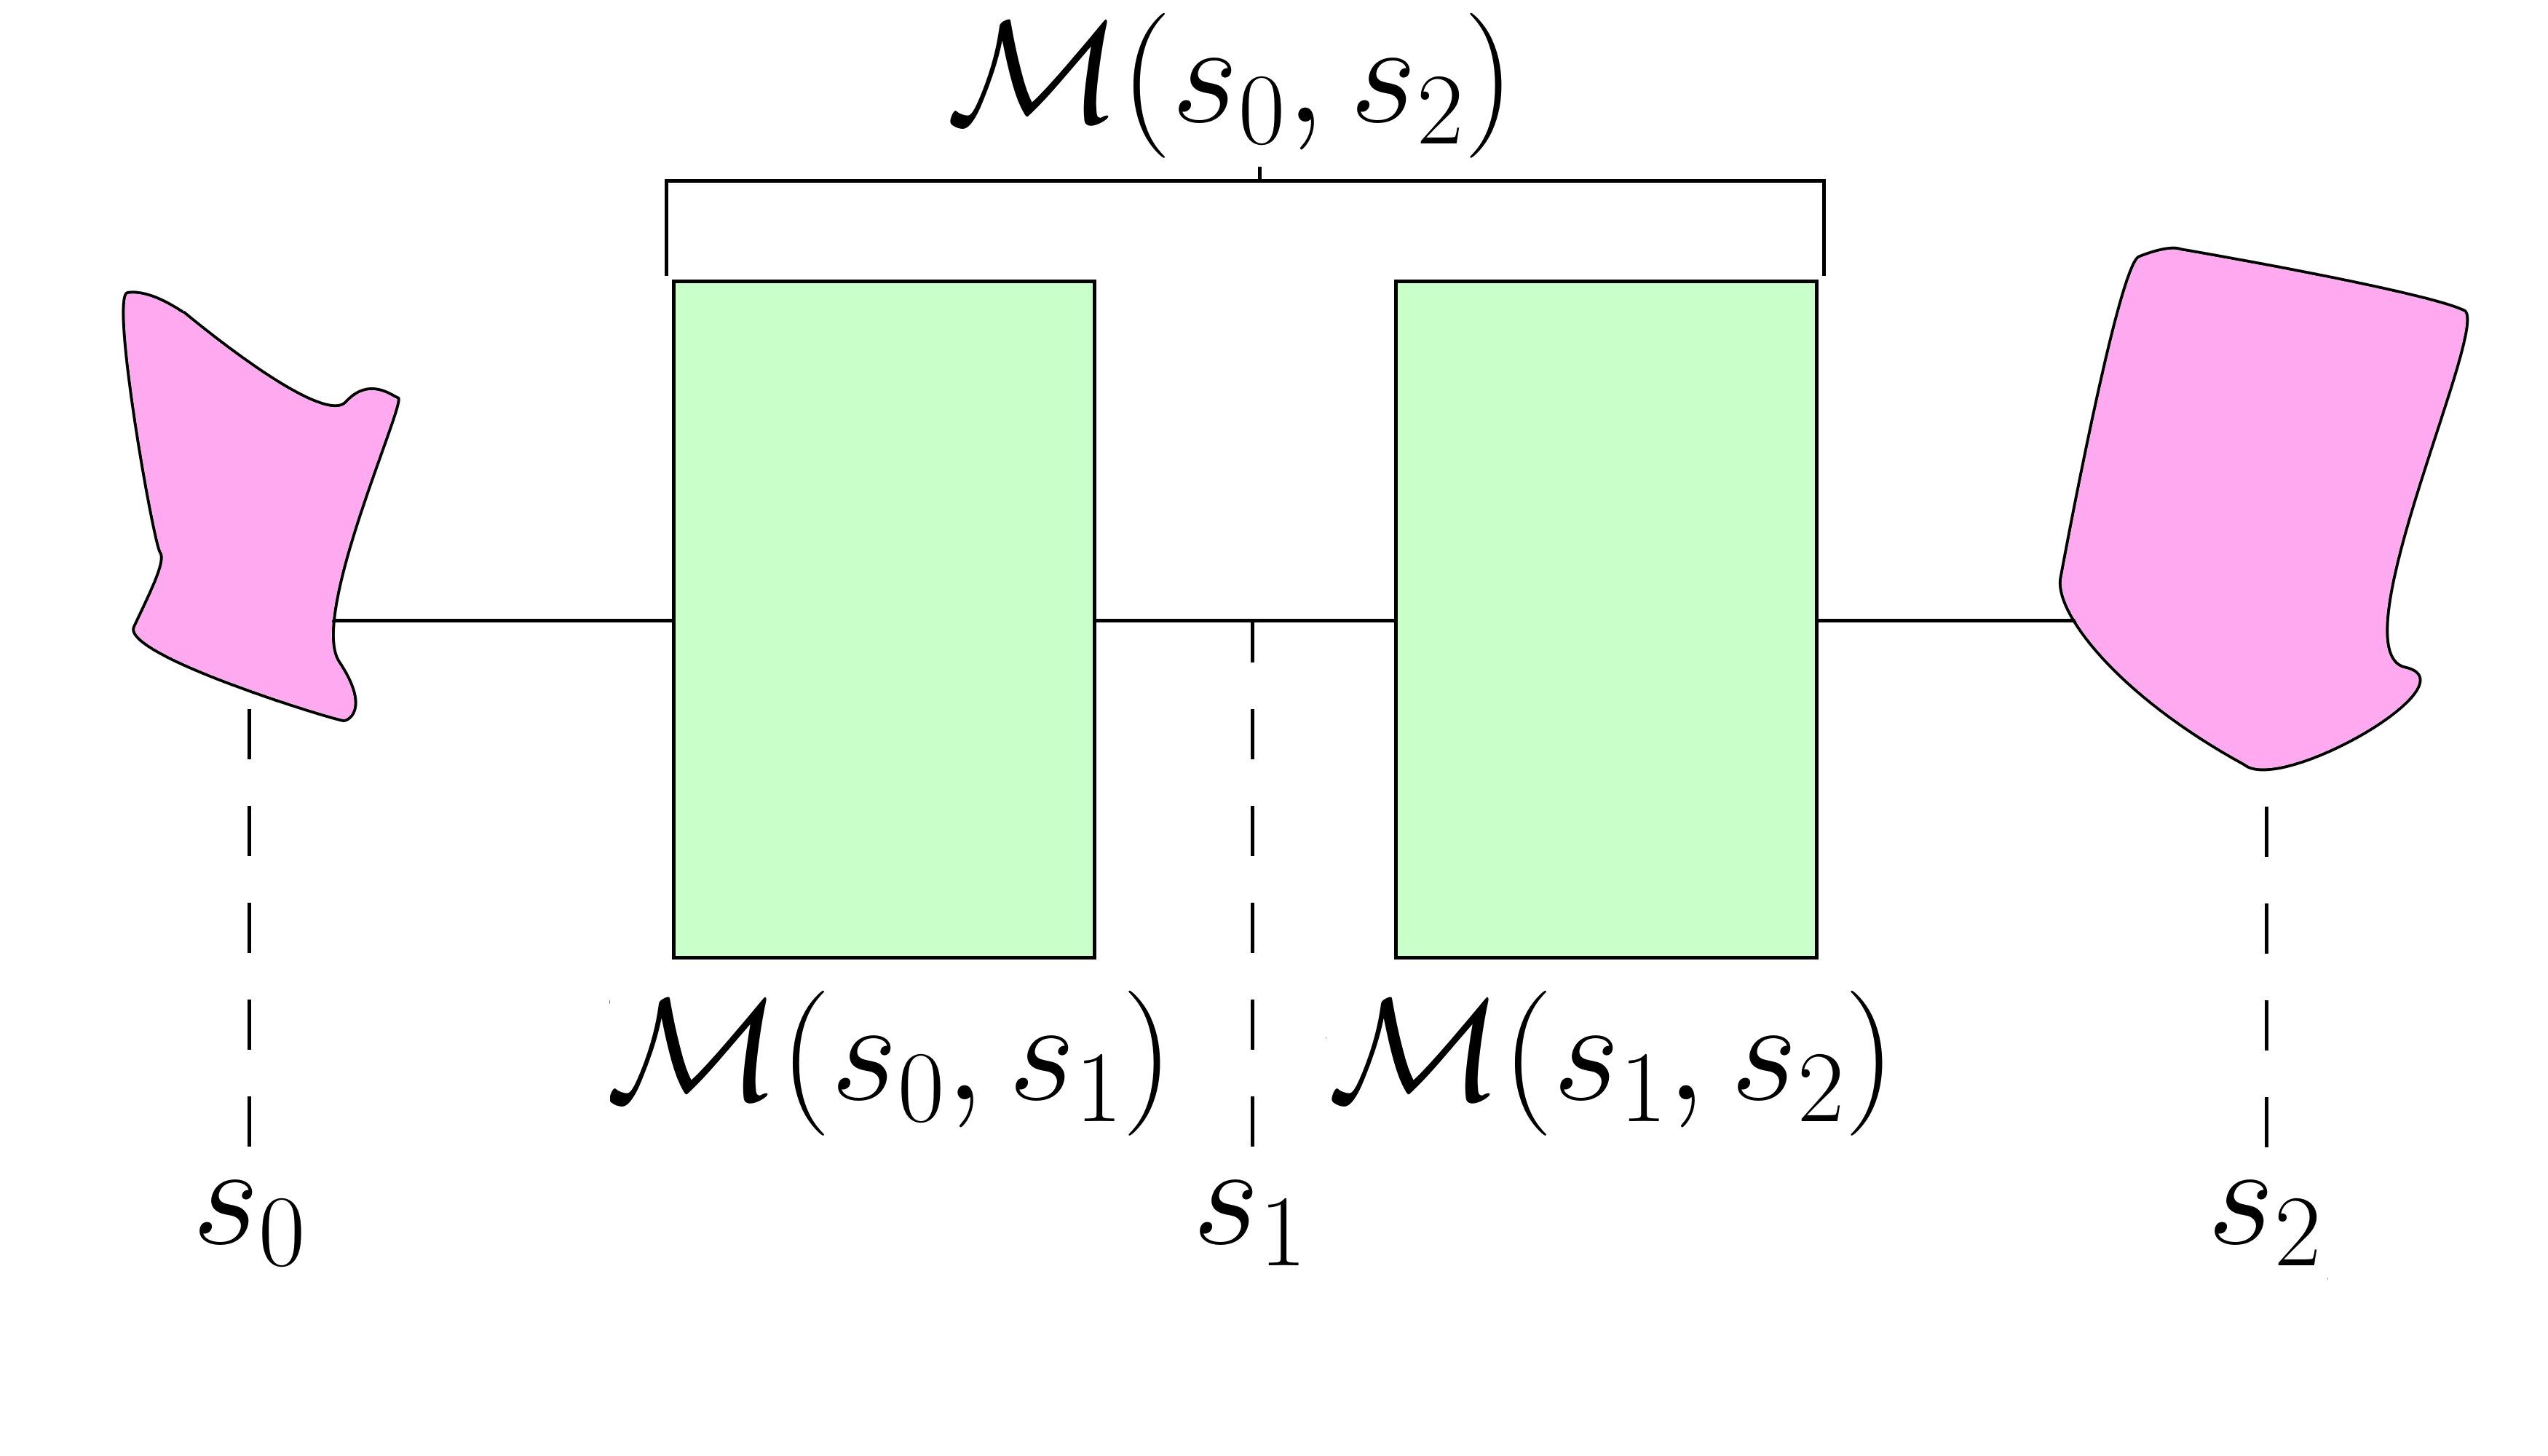
\includegraphics[width=0.75\textwidth]{Figures/matrix_element_example_2} 
  \caption{Example of two maps $\mathcal{M}(s_0,s_1)$ and $\mathcal{M}(s_1,s_2)$. These two maps may be multiplied together to reduce to a single map, $\mathcal{M}(s_0,s_2)$.}
  \label{fig:matrix_element_example_2}
\end{figure}
% Figure at the end of the section is bad!

%-------------------------------------------------------------------------------
\Section{Introduction to Matter-Dominated Lattices}\par

\Subsection{Introduction to Stochastic Effects}\par
This next section introduces stochastic effects, or effects which are intrinsically random. These are not to say effects which are deterministic, but approximated as random, as is the case in classical thermodynamics. In classical thermodynamics, a system has a very large number of particles. These particles and their evolution through time may be kept track of by a set of deterministic interactions (computational biophysics does this well with protein folding), but classically they are approxmated simply as a random set. In this sense, the large thermodynamic system is not stochastic, since it fails to be \emph{intrinsically} random. This is not the case with computational beam physics, as the models involved are typically require close range, dissipative forces, and quantum effects. It's not that the interactions are deterministic but difficult to keep track of, for that would require better bookkeeping or more precise measurements; rather the interactions are random by nature, deterministically unpredictable by no fault of the observer.

As discussed in the next section, this work is concerned with the interactions between a muon beam and some stationary target called the `absorber' --typically a cylinder or wedge filled with liquid hydrogen. The simplest model of a beam interacting with some stationary target can be found in several textbooks \cite{nielsen,griffithsqm}, but perhaps the most helpful model comes from \cite{jose} in Figure \ref{fig:scatteringmodel}.

\begin{figure}
  \centering
  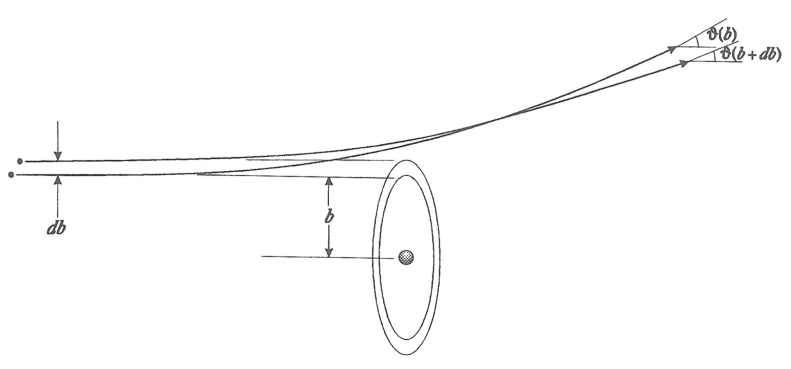
\includegraphics[width=\textwidth]{Figures/scattering_model} 

  \caption{Classical muon--target interaction model courtesy of \cite{jose}.}
  \label{fig:scatteringmodel}
\end{figure}

Here $b$ is referred to as the impact parameter and is measured with respect to the particle's initial trajectory. For a beam of noninteracting particles and a perfectly stationary target, classical mechanics suggest that this is a purely deterministic problem (see, e.g., `hard-sphere scattering' in \cite{griffithsqm}); the particle with a smaller impact parameter $b$ will deflect more than its neighbor with a slightly larger impact parameter of $b+db$. This model is entirely based on initial conditions, and if this were reality it would be relatively easy to implement these effects into the map methods of COSY Infinity. However, reality does not follow the model of Figure \ref{fig:scatteringmodel}. A more accurate model is illustrated by Figure \ref{fig:scatteringmodel2}. Here the target is still approximated as fixed, but the incident particle is now approximated as a travelling plane wave and the scattered particle is approximated as a spherical wave (at least locally).
\begin{figure}
  \centering
    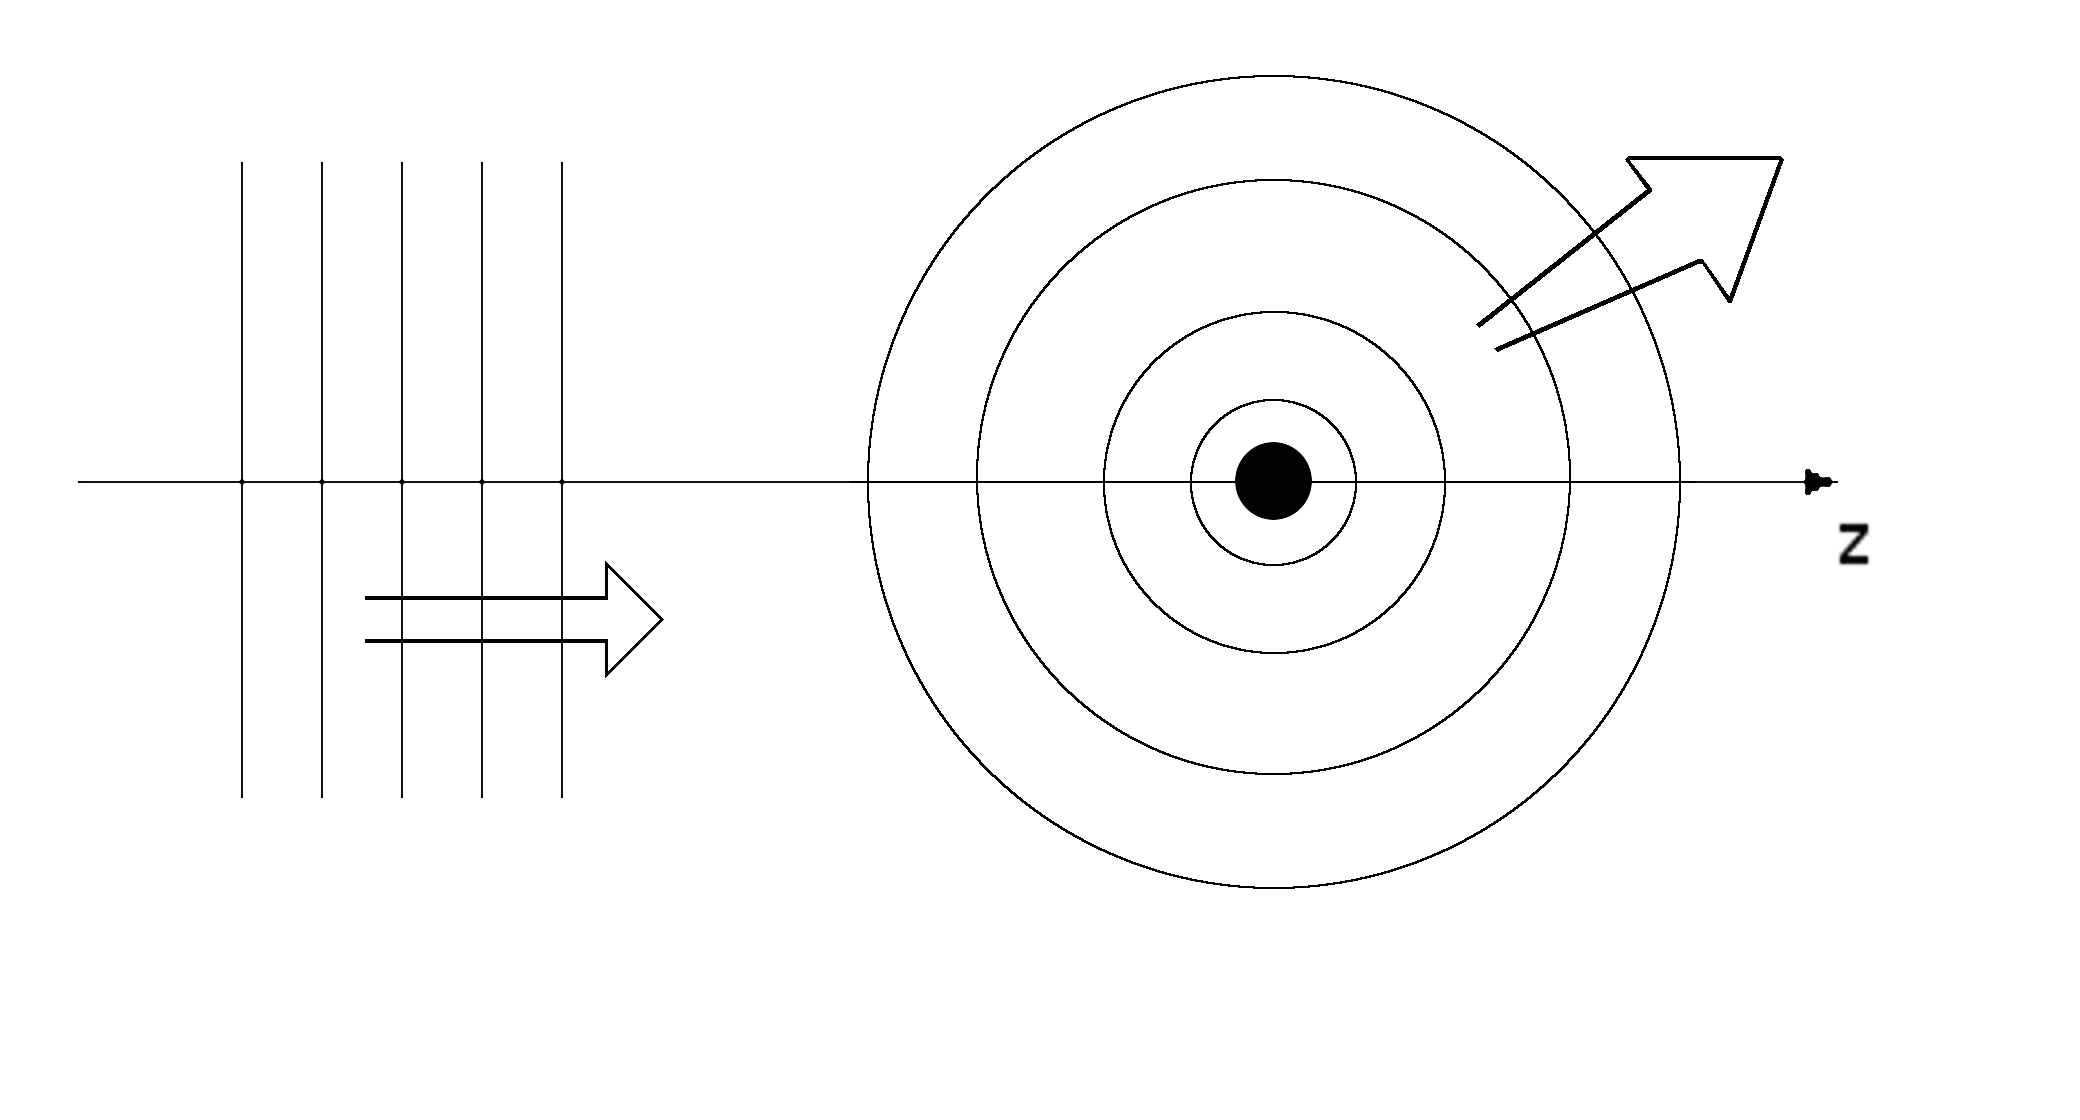
\includegraphics[width=\textwidth]{Figures/scattering_model_2} 
  \caption{Quantum muon-target interaction model. The incoming particle wavefunction is represented as a plane wave and is scattered locally as a spherical wave. Image courtesy of \cite{griffithsqm}.}
  \label{fig:scatteringmodel2}
\end{figure}
It will be shown later that this model predicts 
\begin{enumerate}
\item a spectrum of energy loss $\omega(\epsilon)$ which yields the probability of losing an amount of energy $\epsilon$ (see Section \ref{sec:ICOOLStraggling}), and
\item a scattering amplitude which gives the form of the probability of scattering in a given direction $\theta$ (see Section \ref{sec:ICOOLScattering}).
\end{enumerate}
Hence quantum theory suggests that even if two identical particles have identical initial conditions their final conditions will not be the same.

\Subsection{Muon Ionization Cooling}
In Section 1.1, the only real disadvantage to any muon-based accelerator was the mean muon rest frame lifetime (2 $\mu$s). This is expected to be far too short of a timespan to be useful in a traditional accelerator scheme. For the moment, observe the two proposed schematics in Figure \ref{fig:muon_accelerator_schematic}. The section labelled `Proton Driver' produces the source protons, which will eventually produce muons. This is essential since muons do not naturally occur in great quantities at a convenient extraction point. These protons then strike some large target (which must be optimized to produce the highest yield), resulting in a spray of protons, muons, electrons, and pions (even shorter-lived particles consisting of a quark-antiquark pair). To further optimize this process, it is advantageous to let the pions decay into muons via $\pi^\pm \rightarrow \mu^\pm + \nu_\mu$. The large assemblage of muons is then split up into bunches and propagated through the phase rotator. The next section is where all of the interesting physics lies, and is the topic of this entire thesis. For now, it will be simply addressed as the `cooling channel' and delved into later. Cooling simply means to reduce the bunch's transverse phase space --that is, it means to limit the beam's immediate physical size and possible future physical size in the transverse direction. The purpose of this is to increase the luminosity of the resulting beam; for a collider, this means more collisions; for a neutrino factory, this means more neutrino counts in the detectors (since neutrinos are neutral, the $\nu$ beam would otherwise tend to disperse). After this critical step, the beam accelerates to an appropriate energy. For a neutrino factory, this is 5 GeV, and the muon and antimuon beams are allowed to decay in a storage ring. For a muon collider, the center-of-momentum energy is $\sim$ 126 GeV for a Higgs factory or up to 10 TeV with current technology for high energy studies.

\begin{figure}
  \centering
    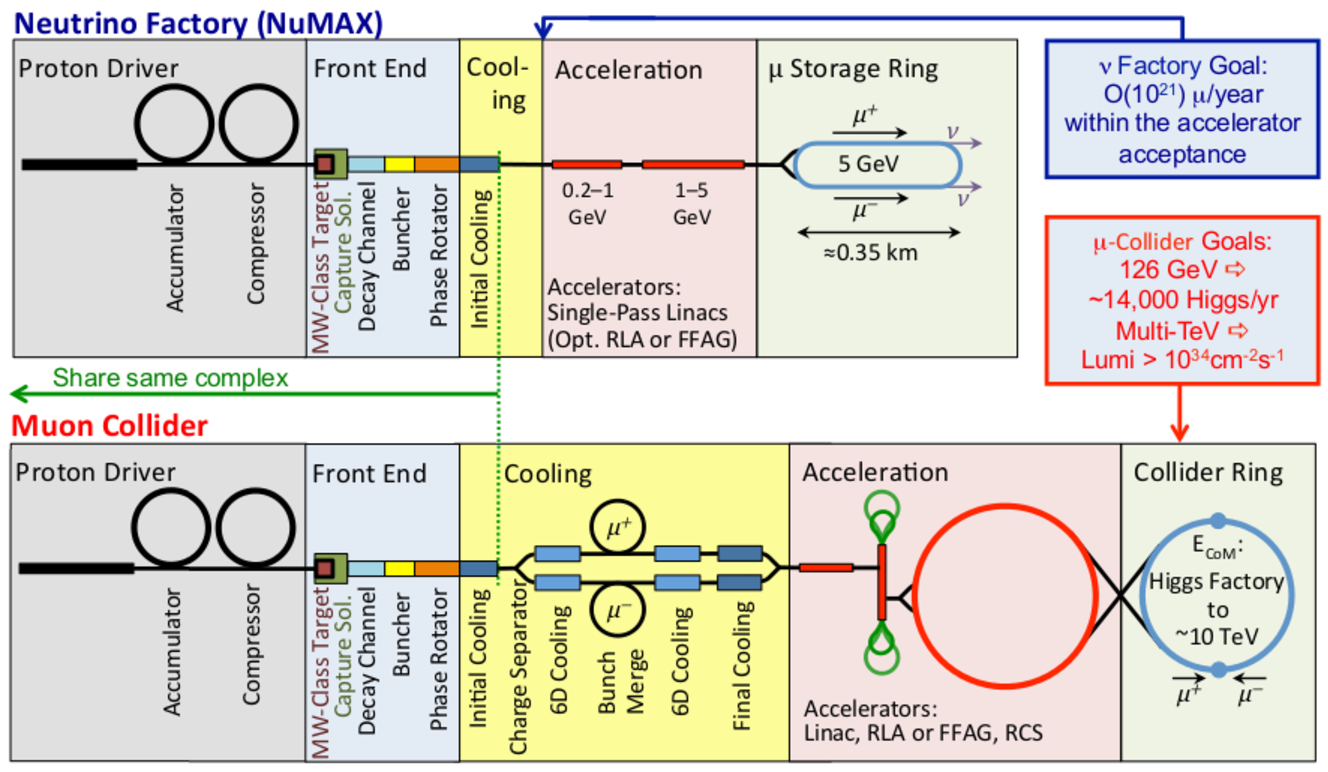
\includegraphics[width=\textwidth]{Figures/muon_accelerator_schematic} 
  \caption{Proposed muon accelerator shematics.}
  \label{fig:muon_accelerator_schematic}
\end{figure}


The cooling channel is the crux of the entire operation for either purpose. Traditional cooling methods (e.g. FODO, electron cooling, etc.) are expected to take far too long to allow a significant portion of the muon beam to survive. For example, for 1 $TeV$ muons the mean muon lifetime in the lab frame is $\bar{t'}=2.2 \mu s$ $\cdot$ 1 $TeV/$ 105.7 $MeV \approx 0.02s$.
 However, ionization cooling is a much faster method. Ionization cooling requires the beam to deposit its energy in matter, thus ionizing the matter. This reduction of total energy in the beam diminishes its phase space in all three directions: ($x, P_x$), ($y, P_y$), and ($z, P_z$). For this reason, it is sometimes also called 6D cooling. 

While the idea of ionization cooling has been around since at least 1956 \cite{oneill,lichtenberg}, it did not appear to be a viable option until roughly 1970 \cite{YuM}. It was believed that the multiple scattering effect would mask any cooling benefits. Scattering is a quantum effect which deflects two objects when they are in close proximity at high energies, and hence is intrinsically random. This means that while the energy deposition reduced the beam's phase space, the beam would also grow in the transverse direction due to this multiple scattering. This phenomenon is now known as phase space exchange or emittance exchange.

Now, this seems to be quite the opposite of what is intended; ionization cooling produces a slow, fat beam, and a good muon beam should be narrow and fast so that the Lorentz boost keeps the muons from decaying. Fortunately, there exists a schematic that solves both of these problems simultaneously. Physically, it is represented in  Figure \ref{fig:coolingchannel} and it is vectorally depicted in Figure \ref{fig:123ionization}.
\begin{figure}
  \begin{center} 
    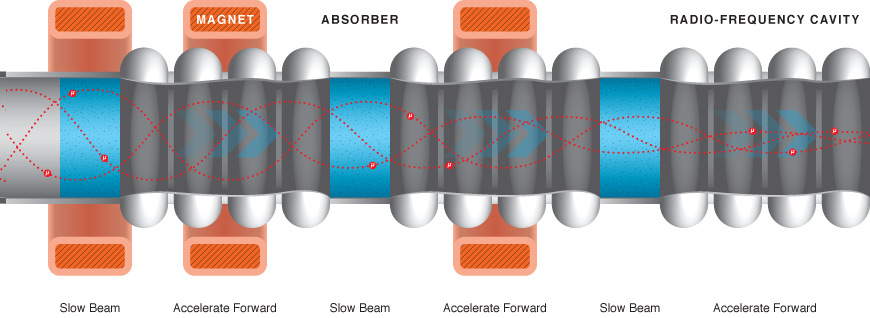
\includegraphics[width=\textwidth]{Figures/coolingchannel} 
  \caption{Cartoon of a cooling channel.}
  \label{fig:coolingchannel}
 \end{center}
\end{figure}

The key is to use a cell which contains both the ionizing material and a radio frequency cavity. It is clear why this solves the latter problem: after the beam loses energy, it gains that much energy again, and so the Lorentz boost stays roughly constant. However, to understand why this solves the former problem it is necessary to observe Figure \ref{fig:123ionization}. In Figure \ref{fig:123ionization}, the longitudinal momentum ($p_l$) is plotted against the transverse momentum ($p_t$). 
   \begin{enumerate} 
  \item{Beam deposits energy in material, reducing the momentum in both directions.}
  \item{Multiple scattering effects are observed. The transverse direction increases (or `heats up'). }
  \item{The beam is re-accelerated by the RF cavity, increasing the longitudinal momentum only. The result is a reduction in transverse momentum (i.e. blue vector compared to black vector).}
\end{enumerate}

\begin{figure}
  \centering
   \captionsetup{singlelinecheck=off}
    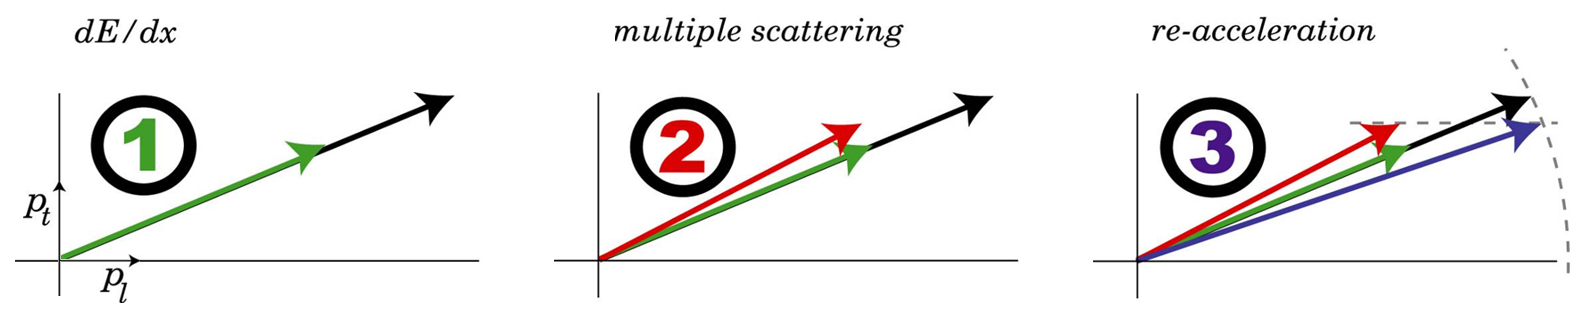
\includegraphics[width=\textwidth]{Figures/123ionization} 
  \caption{Vectoral depiction of ionization cooling in Figure \ref{fig:coolingchannel}. }
  \label{fig:123ionization}
\end{figure}

%-------------------------------------------------------------------------------------------------------------------------------------------------

\Subsection{Emittance}
Often, it is advantageous to represent the volume of phase space occupied by the beam as the emittance, $\epsilon$. Moreover, this volume should be normalized by the usual relativistic factors, $\gamma$ and $\beta$. For the relevant transverse emittance,
%
\begin{equation}
\label{eqn:emittancedef}
%\epsilon_x^N=\beta\gamma\epsilon_x=\beta \gamma\sigma_x \sigma_\theta.
\epsilon_x^N=\beta\gamma\epsilon_x=\beta\gamma\sqrt{\left<x^2\right>\left<\theta^2\right>-\left<x\theta\right>^2}.
\end{equation}
%
Here, azimuthal symmetry is assumed, and so $x$ represents the general transverse position, and $\theta$ is the projection of the divergence angle of the particle trajectory onto the $x$-$z$ plane. 

It is conceptually easy to understand why this represents a volume of phase space. Since the `beam' is a collection of particles, its full width is not simply defined. For this reason, the width of the beam is represented as the beam's RMS. Provided that the beam is nearly Gaussian, if there existed no cross-dependence in $x$ and $\theta$, then the picture should look like the left side of Figure \ref{fig:ellipses}. Then the volume of this bivariate Gaussian is proportional to $\sqrt{\left<x^2\right>\left<\theta^2\right>}$. However, if there is some cross-dependence (right side of Figure \ref{fig:ellipses}) then this must be accounted for by subtracting the cross term from the RMS terms.

\begin{figure}
  \begin{center}
    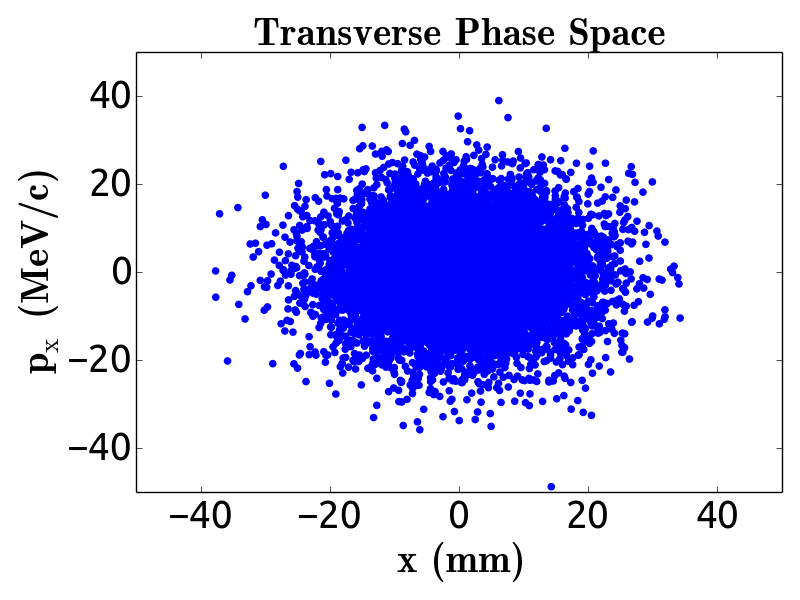
\includegraphics[width=0.49\textwidth]{Figures/ellipse0} 
    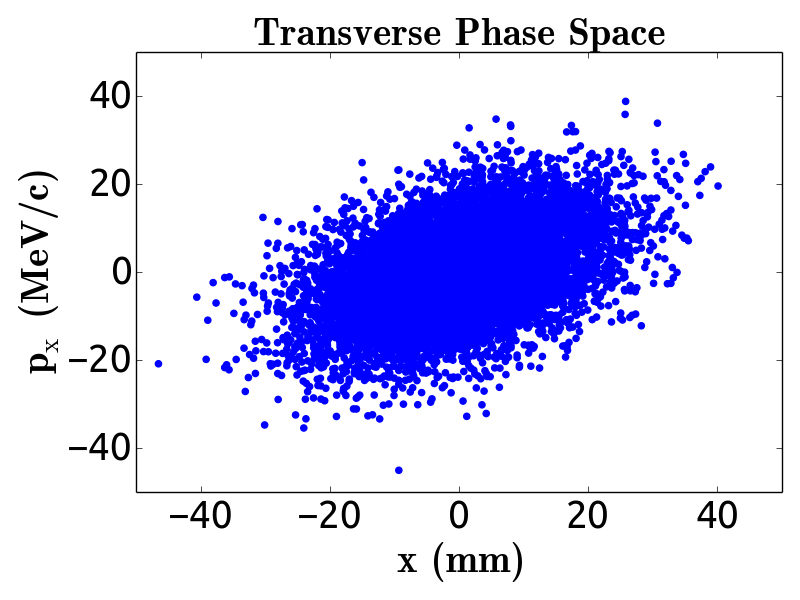
\includegraphics[width=0.49\textwidth]{Figures/ellipse1} 
  \caption{Left: example beam with no $x$-$\theta$ correlation. Right: example beam with significant $x$-$\theta$ correlation.}
  \label{fig:ellipses}
 \end{center}
\end{figure}

Now it is possible to derive the effect of cooling absorbers on emittance as it pertains to muon ionization cooling. Closely following \cite{Fernow}, Eqn. \ref{eqn:emittancedef} is differentiated by $z$:
%
\begin{equation}
\label{eqn:emittance1}
\frac{d\epsilon_x^N}{dz}=\epsilon_x \frac{d(\beta\gamma)}{dz}+\beta\gamma\frac{d\epsilon_x}{dz},
\end{equation}
%
It will soon be shown that the first term represents `cooling' and the second term represents `heating' in the transverse plane. Starting with the heating term,
%
\begin{equation} \nonumber
\frac{d\epsilon_x^N}{dz}(heat)=\beta\gamma\frac{d\epsilon_x}{dz}.
\end{equation}
%

It can be assumed that the cooling is taking place near the beam waist (that is, the part of the trajectory where the beam is smallest). For this case, it is a reasonable approximation that the transverse phase space looks more similar to the left side of Figure \ref{fig:ellipses}, and so the $\left<x\theta\right>$ term may be neglected. Furthermore, with strong focusing it is possible to neglect the rate of position growth of the beam (this is cited in \ref{Fernow} provided the conditions that $\sigma_{xo}^2 \gg \theta_c^2 L / 2\omega^2$ and $\sigma_{xo}^2 \gg \theta_c^2 / 4\omega^3$, where L is the absorber length, $\omega$ is the focusing strength parameter, $\sigma_{xo}$ is the original beam size incident upon the absorber, and $\theta_c$ is the coefficient of the RMS scattering angle given in \cite{highland}). Using these two approximations, the only derivative in the heating term is that by $\left<\theta^2\right>$:
\begin{equation} \nonumber
\frac{d\epsilon_x^N}{dz}(heat)\approx\beta\gamma\frac{d}{dz}\sqrt{\left<x^2\right>\left<\theta^2\right>}\approx \frac{\beta\gamma}{2\epsilon_x}\left<x^2\right>\frac{d}{dz}\left<\theta^2\right>.
\end{equation}

From betatron focusing theory, $\left<x^2\right>$ may be rewritten as $\beta_\perp \epsilon_x$. Moreover, using \cite{highland} $\left<\theta^2\right>$ can be written as $h(z)/\beta^2E$. Here, $h(z)$ is the Highland $z$-dependence, the form of which many theories disagree. However, the first order term of $h(z)$ is generally not model-dependent, and so this becomes
\begin{equation} \nonumber
\left<\theta^2\right>\approx\frac{E_s}{\beta^2 E}\sqrt{\frac{z}{X_0}},
\end{equation}
where $E_s$ is some characteristic energy ($\approx14$ $MeV$) and $X_0$ is the radiation length of the given material. Then
\begin{equation} \nonumber
\frac{d\epsilon_x^N}{dz}(heat)\approx\beta\gamma\frac{\beta_\perp}{2}\frac{d}{dz}\big(\frac{E_s}{\beta^2 E}\sqrt{\frac{z}{X_0}}\big),
\end{equation}

\begin{equation}
\label{eqn:emittanceheat}
\frac{d\epsilon_x^N}{dz}(heat)\approx\frac{\beta_\perp}{2}\frac{E_s^2}{\beta^3Emc^2}\frac{1}{X_0}.
\end{equation}

Now it is clearer why this is referred to as the heating term. Since the derivative of emittance is positive, this part represents emittance growth. Moreover, to reduce this growth it is necessary to have highly energetic particles through a material with a large radiation length (typically $X_0 \propto Z$ (nuclear charge)).

Observe the cooling term of Eqn. \ref{eqn:emittance1}:
\begin{equation} \nonumber
\frac{d\epsilon_x^N}{dz}(cool)=\epsilon_x\frac{d(\beta\gamma)}{dz}=\epsilon_x\cdot(\beta\frac{d\gamma}{dz}+\gamma\frac{d\beta}{dz}).
\end{equation}
First,
\begin{equation} \nonumber
\frac{d\beta}{dz}=\frac{d}{dz}(1-\gamma^{-2})^{\frac{1}{2}}=\frac{1}{\beta\gamma^3}\frac{d\gamma}{dz},
\end{equation}
and then,
\begin{equation} \nonumber
\frac{d\gamma}{dz}=\frac{\gamma}{E}\frac{dE}{dz},
\end{equation}
with $E$ as the total energy of the muon beam. Finally,
\begin{equation} \nonumber
\frac{d\epsilon_x^N}{dz}(cool)=\epsilon_x\cdot(\beta\frac{d\gamma}{dz}+\gamma\frac{1}{\beta\gamma^3}\frac{d\gamma}{dz})=\epsilon_x\cdot\frac{d\gamma}{dz}\beta(1+\frac{1}{\beta^2\gamma^2}) \vspace*{12pt}
\frac{d\epsilon_x^N}{dz}(cool)=\epsilon_x\frac{dE}{dz}\frac{\gamma}{E\beta}.
\end{equation}
Normalizing the emittance by first multiplying and then dividing by $\beta\gamma$ results in
\begin{equation} \nonumber
\frac{d\epsilon_x^N}{dz}(cool)=\frac{1}{\beta}\frac{dE}{dz}\frac{\epsilon_x^N}{E}
\end{equation}
However, there are two notations which should be observed. First, even for a perfect monoenergetic pencil beam energy loss is stochastic, not deterministic. Two muons with identical initial conditions will likely lose different amounts of energy as they pass through the same medium. Since emittance is a collective effect, is it more appropriate to talk about an average energy loss, which turns $\frac{dE}{dz}$ into $\left<\frac{dE}{dz}\right>$. The second observation is with regard to sign convention. Typically, one refers to energy loss as a positive quantity (e.g. the beam lost 10 MeV from point A to point B), even though it is clear that $\frac{dE}{dz}$ is a negative quantity. For this reason, the energy loss term must again be changed from $\left<\frac{dE}{dz}\right>$ to  $-\left|\left<\frac{dE}{dz}\right>\right|$. This leaves the full cooling term as
\begin{equation}
\label{eqn:emittancecool}
\frac{d\epsilon_x^N}{dz}(cool)=-\frac{1}{\beta}\left| \left<\frac{dE}{dz}\right>\right| \frac{\epsilon_x^N}{E}.
\end{equation}

Similar to the heating term, it is now understandable why this is referred to as the cooling term. The rate of change of the normalized transverse emittance is negative, and so the transverse phase space shrinks. However, at this point Eqn. \ref{eqn:emittancecool} does not explain precisely how the rate changes, and so is purely conceptual for the time being. The shape of the cooling term is determined by the average energy loss, $\left|\left<\frac{dE}{dz}\right>\right|$. However, usually it is not $\left|\left<\frac{dE}{dz}\right>\right|$ that is measured, but rather the stopping power $S(E)=-\frac{1}{\rho}\left<\frac{dE}{dx}\right>$, typically in units of $MeV$ $cm^2/g$. A good example of a stopping power curve can be seen in Figure \ref{fig:bethecurve} \cite{PDG}. For this example, there are several effects noted in Figure \ref{fig:bethecurve}, and one may be tempted to think that based on \ref{eqn:emittancecool} the most cooling should occur in the Anderson-Ziegler regime at $\beta\gamma\sim0.01$ (since there is a $1/E$ dependence in Eqn. \ref{eqn:emittancecool}, the high energy part of the curve does no good). Indeed, for $\rho= 8.92$ $g/cm^3$ it is easy to see that at $\beta\gamma=0.01$ then $\frac{d\epsilon_x^N}{dz}(cool)\approx-900$  $cm^{-1} \cdot \epsilon_x^N$ .

However, the correct strategy is just the opposite --one should endeavor to build a cooling cell with the minimum ionization point in mind (in the Bethe regime, where $\beta\gamma\sim2$). At the peak ($\beta\gamma\sim0.01$), the muon beam slows down quite a bit through a single cooling cell and one is at risk of losing their beam to decay. Moreover, Figure \ref{fig:bethecurve} only depicts the stopping power, not the actual energy loss that individual particles experience. The individual energy loss is a stochastic effect, and the distribution of energy losses broadens with decreasing beam energy. This means that for lower energies, there will be more particles which stop completely. Further, with a higher beam energy the stochastic energy loss profile is more sharply peaked, and so there are fewer decays and more particles which fall into the RF bucket. (Remember, the longitidunal emittance is observed by the RF cavities, as seen in Figure \ref{fig:coolingchannel}. The longitudinal emittance increases with energy loss according to \cite{Fernow}.) Finally, it is apparent in Eqn. \ref{eqn:emittanceheat} that higher energies are better, since they reduce the heating term. For these reasons, it is apparent that a muon cooling cell should be made of low $Z$ materials such as liquid hydrogen or lithium hydride and operate anywhere between 100 $MeV$/c to 400 $MeV$/c.

\begin{figure}
  \centering
    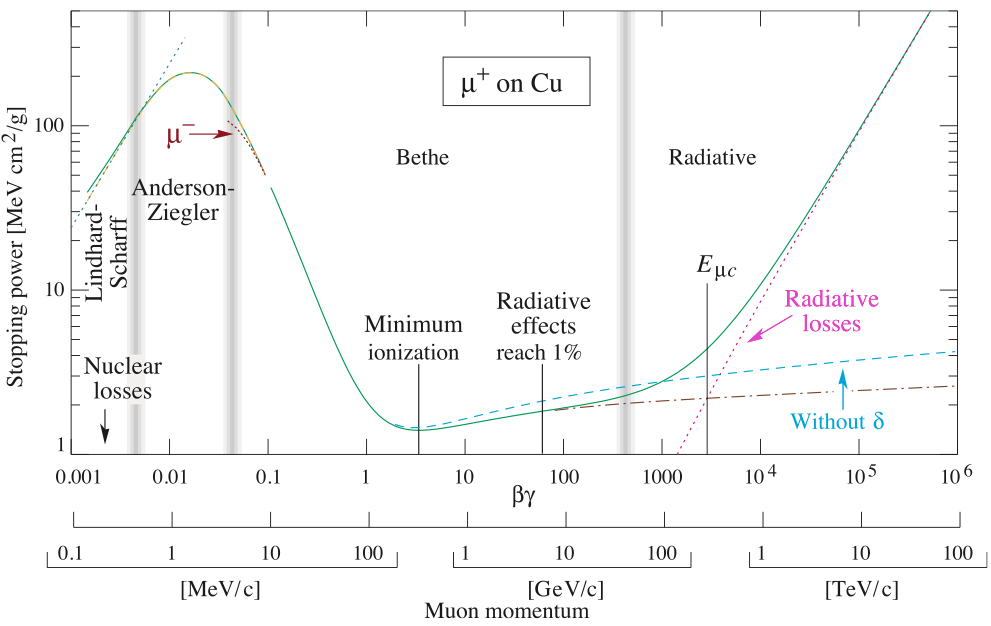
\includegraphics[width=\textwidth]{Figures/bethecurve} 
  \caption{Stopping power curve for antimuons on copper, courtesy of \cite{PDG}. }
  \label{fig:bethecurve}
\end{figure}

When particles impinge upon a fixed target, they lose some of their energy. For massive particles like muons, there are four major effects which contribute to this energy loss: ionization, bremsstrahlung radiation, pair production, and photonuclear interactions. However, it is important to note that in the muon cooling regime only ionization contributes significantly to the energy loss. To see this, take for an example the relatively heavy element of iron (iron is chosen because it is a fairly relatable element to those who are not experts in this field). In Figure \ref{fig:elossfe}, the energy loss contributions of these four effects can be seen. However, the non-ionization effects only start to contribute at an initial beam kinetic energy of 1.40 $GeV$ --far outside of the muon cooling regime.

\begin{figure}
  \centering
    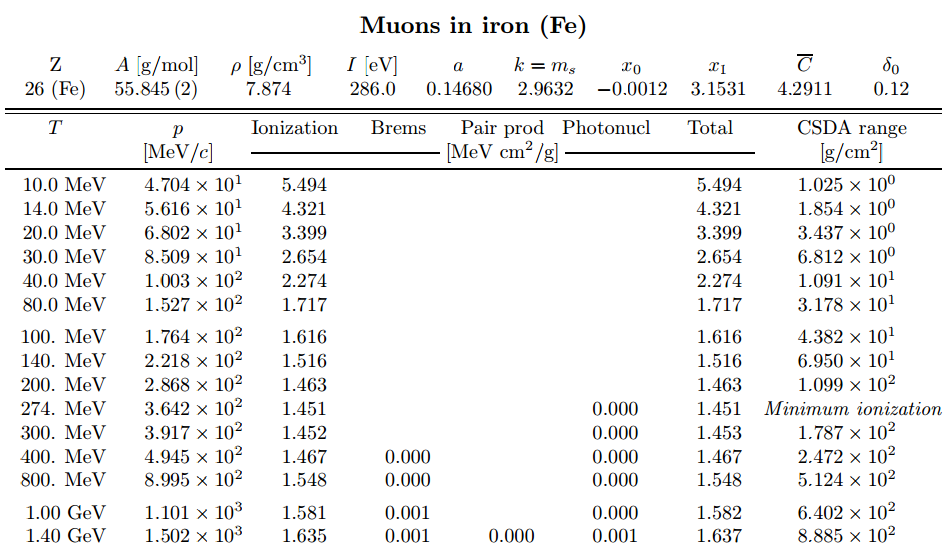
\includegraphics[width=\textwidth]{Figures/E_loss_Fe} 
  \caption{Energy loss table for muons in iron. Table courtesy of \cite{PDGTables}.}
  \label{fig:elossfe}
\end{figure}

This is a good example because all of the cooling materials currently being considered have less muon stopping power than iron. This means that iron represents the maximum contribution of non-ionization energy loss per initial beam energy; that is, the non-ionization effects begin to emerge at much higher energies for lighter elements such as liquid hydrogen. Note that Figure \ref{fig:bethecurve} may also be useful when discussing this subject.

Here, \textit{ionization} refers to both true ionization (the production of $\delta$ rays) and excitation (the promotion of an inner electron to a higher shell). To reiterate a previous section, the term `straggling' refers to the fluctuation about some mean energy loss. That is to say, the amount of energy that a particle will lose is intrinsically random --there exists some distribution with some average value, and when the particle of interest transverses a length of matter the amount of energy that this particle loses is selected from this distribution. This intrinsic randomness can be attributed to quantum-like behaviors (e.g. the energy loss cross section which comes from the wave nature of the particle in question).